%%=============================================================================
%% Methodologie
%%=============================================================================

\chapter{\IfLanguageName{dutch}{Methodologie}{Methodology}}%
\label{ch:methodologie}

% Door de vergaarde kennis uit de literatuurstudie in hoofdstuk \ref{ch:stand-van-zaken} over de mogelijke noden van scholieren met dyslexie, de complexiteit van wetenschappelijke artikelen, de technieken voor MTS en ATS, en de bijhorende valkuilen bij taalverwerking met AI, kunnen onderzoeksmethoden worden toegepast om een antwoord te vinden op de onderzoeksvraag. 

Om een antwoord te vormen op de onderzoeksvraag, moet de vergaarde kennis uit de literatuurstudie in drie onderzoeksmethoden. Eerst staat het onderzoek stil bij de vereiste functionaliteiten om gepersonaliseerde ATS te kunnen realiseren. Vervolgens achterhaalt het onderzoek het geschikte taalmodel voor gepersonaliseerde ATS. Tenslotte volgt de ontwikkeling van een prototype voor ATS-vereenvoudiging van wetenschappelijke artikelen. Zo doelt dit onderzoek om de haalbaarheid voor een toepassing voor gepersonaliseerde ATS te achterhalen aan de hand van een prototype. Dit prototype moet in staat zijn om wetenschappelijke artikelen te vereenvoudigen op maat voor scholieren met dyslexie in de derde graad van het middelbaar onderwijs.

\section{Requirementsanalyse}
\label{sec:requirementsanalyse}

Om het ontwikkelingsproces van het prototype gericht te sturen, moet het onderzoek MTS- en ATS-technologieën in bestaande tools nagaan. Zo gebeurt het verkennen en experimenteren op ATS-technieken bij beschikbare tools door een kwalitatief onderzoek in de vorm van een requirementsanalyse. Het resultaat van deze onderzoeksfase is een Moscow-schema dat de benodigde functionaliteiten voor een toepassing met ATS definieert, met als doel een vergelijkbare toepassing aan te bieden voor gepersonaliseerde ATS van wetenschappelijke artikelen met de kwaliteiten van gepersonaliseerde MTS. Daarnaast achterhaalt de onderzoeksfase de ontbrekende MTS-functionaliteiten die tabel \ref{table:benefits-mts} in de literatuurstudie uitwees. De geteste toepassingen, opgesomd in tabel \ref{table:shortlist-tools}, beschikken over (gepersonaliseerde) ATS-technieken. Deze lijst omvat erkende toepassingen van de overheid en toepassingen die leerkrachten of scholieren kunnen gebruiken om teksten te vereenvoudigen. Met deze onderzoeksmethode kan het onderzoek een antwoord geven op de volgende twee deelvragen van het onderzoek.

\begin{itemize}
	\item Welke functies ontbreken AI-toepassingen om geautomatiseerde tekstvereenvoudiging mogelijk te maken voor scholieren met dyslexie in de derde graad middelbaar onderwijs?
	\item Welke manuele methoden voor tekstvereenvoudiging komen niet in deze tools voor?
\end{itemize}

Figuur \ref{img:flowchart-requirementsanalyse} toont de flowchart om de requirementsanalyse te kunnen uitwerken.

\begin{figure}[H]
	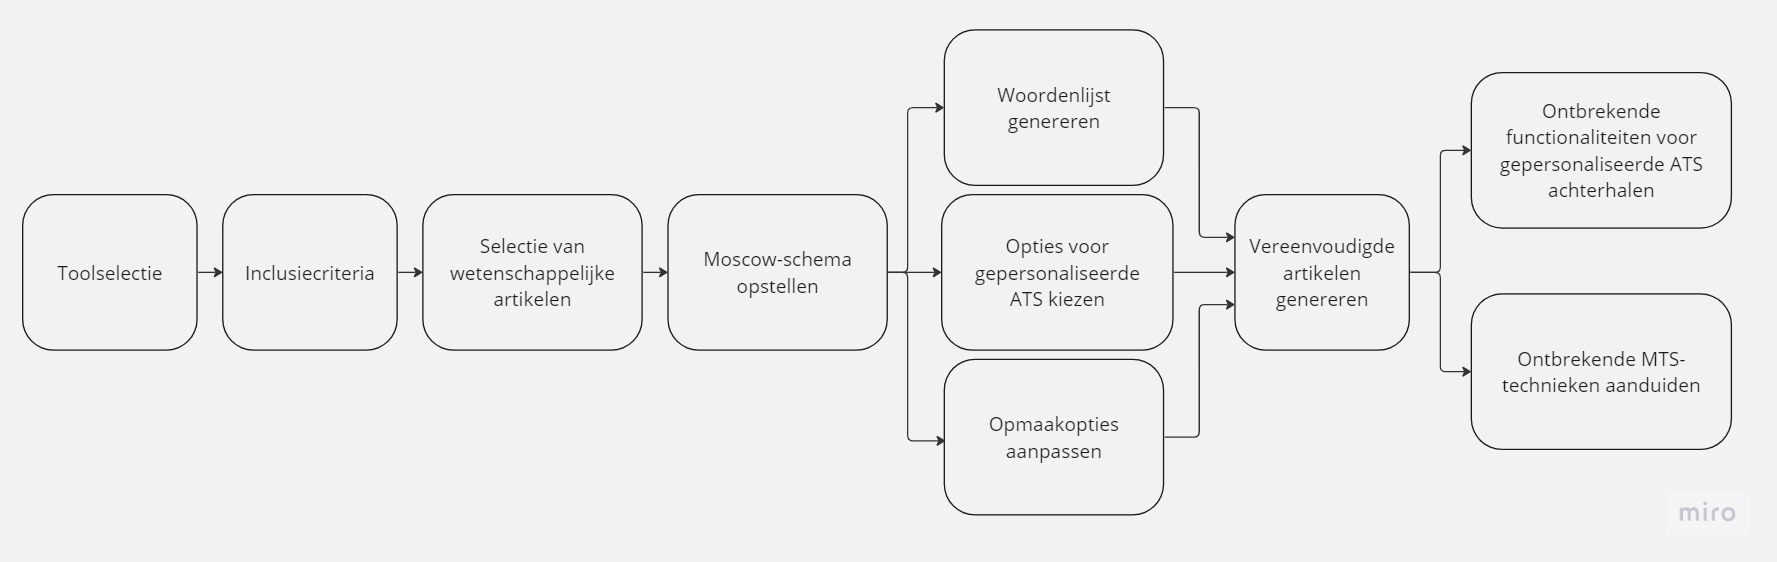
\includegraphics[width=\linewidth]{img/flowchart-requirementsanalyse.jpg}
	\caption{Het benodigde stappenplan bij de requirementanalyse.}
	\label{img:flowchart-requirementsanalyse}
\end{figure}

% TOOLSELECTIE 
Allereerst start het onderzoek met een toolselectie. Zoals aangewezen in sectie \ref{sec:beschikbare-tools-en-taalmodellen}, leent de overheid vijf softwarepakketten uit aan middelbare scholen. Echter neemt de requirementsanalyse drie van deze vijf in de analyse op, want hun functionaliteiten zijn passend voor deze doelgroep. De overige twee zijn minder aanwezig in het onderwijs. Daarnaast toont een zoekopdracht aan dat deze tools geen lexicale vereenvoudiging toepassen. 

Naast deze erkende softwarepakketten kunnen online beschikbare tools ook scholieren met dyslexie ondersteunen bij het begrijpend lezen van wetenschappelijke artikelen met ATS, zoals bewezen in \textcite{Bingel2018}. Daarom betrekt de requirementsanalyse enkel tools met onderschreven ATS-functionaliteiten en laat daarmee pure samenvattingstools erbuiten. Tabel \ref{table:shortlist-tools} toont een overzicht van de te experimenteren tools.

\begin{center}
	\begin{table}[H]
		\begin{tabular}{ | m{6cm} | m{6cm} | } 
			\hline
			\textbf{Erkende software} & \textbf{Online beschikbare tools} \\
			\hline
			Sprintplus (E1) & Simplish (O1) \\
			Kurzweil3000 (E2) & SciSpace (O2) \\ 
			AlineaSuite (E3) & Rewordify (O3) \\
			& ChatGPT (O4) \\
			& Bing Chat (O5) \\
			\hline
		\end{tabular}
		\caption{Shortlist van uit te testen tools en toepassingen voor tekstvereenvoudiging.}
		\label{table:shortlist-tools}	
	\end{table}
\end{center}

% Inclusiecritera
Vervolgens bouwt het onderzoek een lijst op van de toetsingscriteria. Zo dienen de MTS-technieken uit tabel \ref{table:scientific-paper-struggles} en tabel \ref{table:manual-simplification} als bouwstenen voor het opstellen van de toetsingscriteria. Tabel \ref{table:criteria-requirementsanalysis} geeft een opsomming van de MTS-technieken waaraan tools moeten voldoen. Daarnaast dient dit schema om een inschatting van de functionaliteiten van deze tools te maken.

\begin{center}
	\begin{table}[H]
		\begin{tabular}{ | m{4cm} | m{11cm} | } 
			\hline
			\textbf{MTS-techniek} & \textbf{Functionaliteit} \\
			\hline
			Lexicale & Gepersonaliseerde LS, ofwel woordenschat dat niet te hooggegrepen is. Gekende woordenschat mag blijven. \\
			vereenvoudiging & Woorden met minder lettergrepen gebruiken \\
			& Extra uitleg schrijven bij zinnen \\
			& Paragrafen herschrijven zodat ze eerst uitleg geven op een high-level niveau, vervolgens lagen van complexiteit toevoegen om de lezer te begeleiden \\
			& Woordenlijst aanmaken \\
			& Idiomen vervangen door eenvoudigere synoniemen \\
			\hline
			Syntactische & Zinnen inkorten \\
			vereenvoudiging & Verwijswoorden aanpassen \\
			& Voorzetseluitdrukkingen aanpassen \\
			& Samengestelde werkwoorden aanpassen \\
			& Actieve stem toepassen \\
			& Enkel regelmatige werkwoorden gebruiken \\
			\hline
			Structurele & Achtergrondkleur aanpassen \\
			aanpassingen & Woord- en karakterspatiëring \\
			& Consistente lay-out \\
			& Duidelijk zichtbare koppenstructuur \\
			& Huidige positie benadrukken \\
			& Waarschuwingen geven omtrent formulieren en sessies \\
			& Inhoud visueel groeperen \\
			& Tekst herschrijven als tabel \\
			& Tekst herschrijven als opsomming \\
			\hline
		\end{tabular}
		\caption{Richtlijnen waarop het onderzoek de toepassingen aftoetst in de requirementsanalyse.}
		\label{table:criteria-requirementsanalysis}	
	\end{table}
\end{center}

Als realistisch testmateriaal, maken de experimenten gebruik van twee gepubliceerde wetenschappelijke artikelen. Zo kunnen deze artikelen relevant zijn voor leerkrachten om aan scholieren in de derde graad van het middelbaar onderwijs te geven als leesvoer. Beide artikelen volgen de kenmerken van een wetenschappelijk artikel, zoals beschreven in tabel \ref{table:scientific-paper-struggles}. Daarnaast gebruiken ze vakjargon en wetenschappelijke concepten in een compact formaat. Tabel \ref{table:referentieteksten-bronvermelding} geeft een overzicht van de twee artikelen en een bijhorende bronvermelding.

\begin{center}
	\begin{table}[H]
		\begin{tabular}{ | m{10cm} | m{5cm} | } 
			\hline
			\textbf{Titel} & \textbf{Bronvermelding} \\
			\hline
			De controle op het gebruik van algoritmische surveillance- onder druk? Een exploratie door de lens van de relationele ethiek & \autocite{VanBrakel2022} \\
			\hline
			Nederland versus België: verschillen in economische dynamiek en beleid. & \autocite{Sleuwaegen2022} \\
			\hline
		\end{tabular}
		\caption{Bronvermeldingen voor de twee wetenschappelijke artikelen.}
		\label{table:referentieteksten-bronvermelding}
	\end{table}
\end{center}

% 4. 
Om een overzicht te hebben van de functionaliteiten volgens prioriteit, bouwt het onderzoek een Moscow-schema vanuit de opgestelde richtlijnen. Zo komen belangrijke functionaliteiten, die nodig zijn om gepersonaliseerde tekstvereenvoudiging met ATS mogelijk te maken, in de categorie \textit{must-haves} terecht. Alle vereiste functionaliteiten om (gepersonaliseerde) ATS mogelijk te maken, moet als \textit{must-have} in het Moscow-schema voorkomen. Irrelevante functionaliteiten binnen de scope van een prototype of niet toepasselijk voor de doelgroep plaatst het onderzoek als \textit{wont-have}.

\begin{center}
	\begin{table}[H]
		\begin{tabular}{ | m{4cm} | m{11cm} | } 
			\hline
			\textbf{MoSCoW-principe} & \textbf{Functionaliteit} \\
			\hline
			Must-have & Gepersonaliseerde LS, ofwel woordenschat dat niet te hooggegrepen is. Gekende woordenschat mag blijven. \\
			& Woorden met minder lettergrepen gebruiken. \\
			& Woordenlijst aanmaken na handmatige CWI. \\
			& Wetenschappelijke artikelen in PDF-vorm opladen. \\
			& Structurele aanpassingen toepassen op de oorspronkelijke tekst. \\
			& Personaliseerbare opmaakopties, waaronder lettertype -en grootte aanpassen, tekstformaat aanpassen, achtergrondkleur aanpassen. \\
			& Duidelijk zichtbare koppenstructuur. \\
			& Tekst herschrijven als opsomming. \\
			\hline
			Should-have & \\
			& Tekst-analyse \\
			& Extra (in-line) uitleg schrijven bij moeilijke woordenschat. \\
			& Personaliseerbare PDF- of Word-document lay-out. \\
			& Uitvoer als PDF of Word-bestand teruggeven. \\
			& Wetenschappelijke artikelen in PDF-vorm opladen met OCR. \\
			& Tekstanalyse voor en na de vereenvoudiging aanbieden. \\
			\hline
			Could-have 
			& Gebruikersfeedback \\
			& Woordenschat genereren na automatische CWI. \\
			& Huidige positie benadrukken. \\
			& Waarschuwingen geven omtrent formulieren en sessies. \\
			& Enkel regelmatige werkwoorden gebruiken. \\
			& Extraherende samenvatting \\
			& Abstraherende samenvatting \\
			& Tekst herschrijven in tabelvorm \\
			\hline
			Wont-have & \\
			& Mobiele versie of \textit{responsive design}. \\
			& Audio-uitvoer \\
			& Integratie met externe toepassingen, waaronder spelcheckers. \\
			\hline
		\end{tabular}
		\caption{Het Moscow-schema voor de requirementsanalyse.}
		\label{img:moscow-table}
	\end{table}
\end{center}

\medspace

Vervolgens komen experimenten rond de opties rond gepersonaliseerde ATS aan bod. Eindgebruikers moeten wetenschappelijke artikelen kunnen opladen. Eindgebruikers kunnen enkel pdf's inladen bij SprintPlus, Kurzweil3000, AlineaSuite, Simplish, Rewordify en SciSpace. In tegenstelling tot Bing Chat en ChatGPT waarbij \textit{plain-text} of een link naar het wetenschappelijk artikel de enige vormen van invoer zijn. De tekstinhoud uit de PDF extraheren gebeurt dan manueel en deze tekst dient daarna als invoer voor de chatbot. Beide chatbots krijgen de prompt, gevolgd door een stuk van het wetenschappelijk artikel. Met zes verschillende prompts kan het onderzoek de functionaliteit om LS, SS of structurele aanpassingen op een tekst door een toepassing achterhalen. Tabel \ref{table:tested-prompts-requirementsanalysis} vermeldt de toegepaste prompts. Toepassingen krijgen eerst een link van het wetenschappelijk artikel, zoals aangegeven in figuur \ref{img:tryout-bing-ai}. Als de toepassing hier niet over beschikt, dan krijgt de chatbot de tekstinhoud van het wetenschappelijk artikel in \textit{plain-text} mee. 

\begin{center}
	\begin{table}[H]
		\begin{tabular}{ | m{2cm} | m{14cm} | } 
			\hline
			\textbf{Naam} & \textbf{Prompt} \\
			\hline
			P1 & Vereenvoudig deze tekst. \\
			\hline
			P2 & Vereenvoudig deze tekst voor studenten (16-18 jaar) door moeilijke woorden te vervangen, vakjargon te schrappen, woorden langer dan 18 letters te vervangen, acroniemen voluit te schrijven, een woord slechts eenmaal door een synoniem te vervangen, korte uitleg te geven wanneer dat nodig is, en percentages te vervangen. \\
			\hline
			P3 & Vereenvoudig een tekst door deze op te delen in kortere zinnen van maximaal tien woorden. Verander voornaamwoorden als 'zij', 'hun' of 'hij' in namen. Vervang complexe zinsconstructies en voorzetselzinnen door eenvoudiger alternatieven, maar laat ze ongewijzigd als er geen eenvoudiger optie beschikbaar is. \\
			\hline
			P4 & Schrijf de tekst als opsomming. \\
			\hline
			P5 & Schrijf de tekst in tabelformaat. \\
			\hline
			P6 & Genereer op basis van deze tekst een woorden- en synoniemenlijst. \\
			\hline
		\end{tabular}
		\caption{De toegepaste GPT-3-prompts in de requirementsanalyse.}
		\label{table:tested-prompts-requirementsanalysis}
	\end{table}
\end{center}

\medspace

Daarna voert het onderzoek experimenten rond gepersonaliseerde opmaakopties uit. Kurzweil, SprintPlus en AlineaSuite bieden opmaakopties aan in het instellingenscherm. Zo kunnen eindgebruikers het lettertype, -kleur -en grootte en de achtergrondkleur aanpassen naar keuze. Als een toepassing niet over opmaakopties beschikt, dan stopt het experiment rond opmaakopties voor die toepassing.

\medspace

Ten slotte test het onderzoek de capaciteiten om het formaat van teksten aan te passen aan de hand van structurele aanpassingen. Zo vragen P4 en P5 specifiek naar een structurele aanpassing, terwijl P1, P2 en P3 minstens een doorlopende tekst als resultaat verwachten. Andere beschikbare tools missen checkboxen of keuzelijsten om deze keuze aan te reiken, waardoor het testen van deze functionaliteit niet mogelijk is.

\section{Vergelijkende studie}
\label{sec:vergelijkende-studie}

Om wetenschappelijke artikelen met gepersonaliseerde ATS te vereenvoudigen, moet dergelijk toepassing gebruikmaken van een geschikt taalmodel. Zo moet de uitvoer van het prototype een vereenvoudigde versie van een wetenschappelijk artikel kunnen geven, specifiek voor de noden van scholieren met dyslexie in de derde graad van het middelbaar onderwijs. Om de uitvoer van het prototype nauwkeurig af te stemmen, vereist het onderzoek een antwoord op de volgende vraag.

\begin{itemize}
	\item Welk taalmodel is geschikt voor tekstvereenvoudiging met ATS van wetenschappelijke artikelen voor scholieren met dyslexie in de derde graad van het middelbaar onderwijs, met dezelfde of gelijkaardige kwaliteiten als gepersonaliseerde tekstvereenvoudiging met MTS?
\end{itemize}

Er zijn weinig gespecialiseerde taalmodellen beschikbaar om wetenschappelijke artikelen te vereenvoudigen. Daarom beoordeelt de vergelijkende studie alle vermelde taalmodellen opgesomd in tabel \ref{table:vergelijkende-studie-taalmodellen}.

\begin{center}
	\begin{table}[H]
		\begin{tabular}{ | m{4cm} | m{11cm} | } 
			\hline
			\textbf{Verwijzing} & \textbf{Taalmodel} \\
			\hline
			T1 & Haining Scientific Abstract Simplification \\
			\hline
			T2 & BART-based Scientific Lay Summarizer \\
			\hline
			T3 & Keep It Simple\\
			\hline
			T4 & GPT-3 \\
			\hline
		\end{tabular}
		\caption{Gebruikte taalmodellen in de vergelijkende studie}
		\label{table:vergelijkende-studie-taalmodellen}
	\end{table}
\end{center}

De vergelijkende studie bestaat uit vijf fasen, weergegeven op de \textit{flowchart} in figuur \ref{img:flowchart-vergelijkende-studie-metrics}. Zo vergelijkt deze onderzoeksfase de leesgraadscores van de oorspronkelijke wetenschappelijke artikelen zoals in sectie \ref{sec:requirementsanalyse}, met referentieteksten vereenvoudigd met MTS en teksten vereenvoudigd met ATS. Met een \textit{mixed-methods} onderzoek kan de vergelijkende studie taalmodellen beoordelen op objectief en subjectief niveau. 

De gebruikte wetenschappelijke artikelen zijn identiek aan de taalmodellen in tabel \ref{table:referentieteksten-bronvermelding}. Om realistisch referentiemateriaal te verkrijgen, schrijven twee leerkrachten en twee leerlingen zonder dyslexie zelf een vereenvoudiging van de twee wetenschappelijke artikelen met MTS. Deze vier personen baseren zich op vooraf meegekregen richtlijnen, toegelicht in de bijlage \ref{ch:referentietekst}. 

\begin{figure}
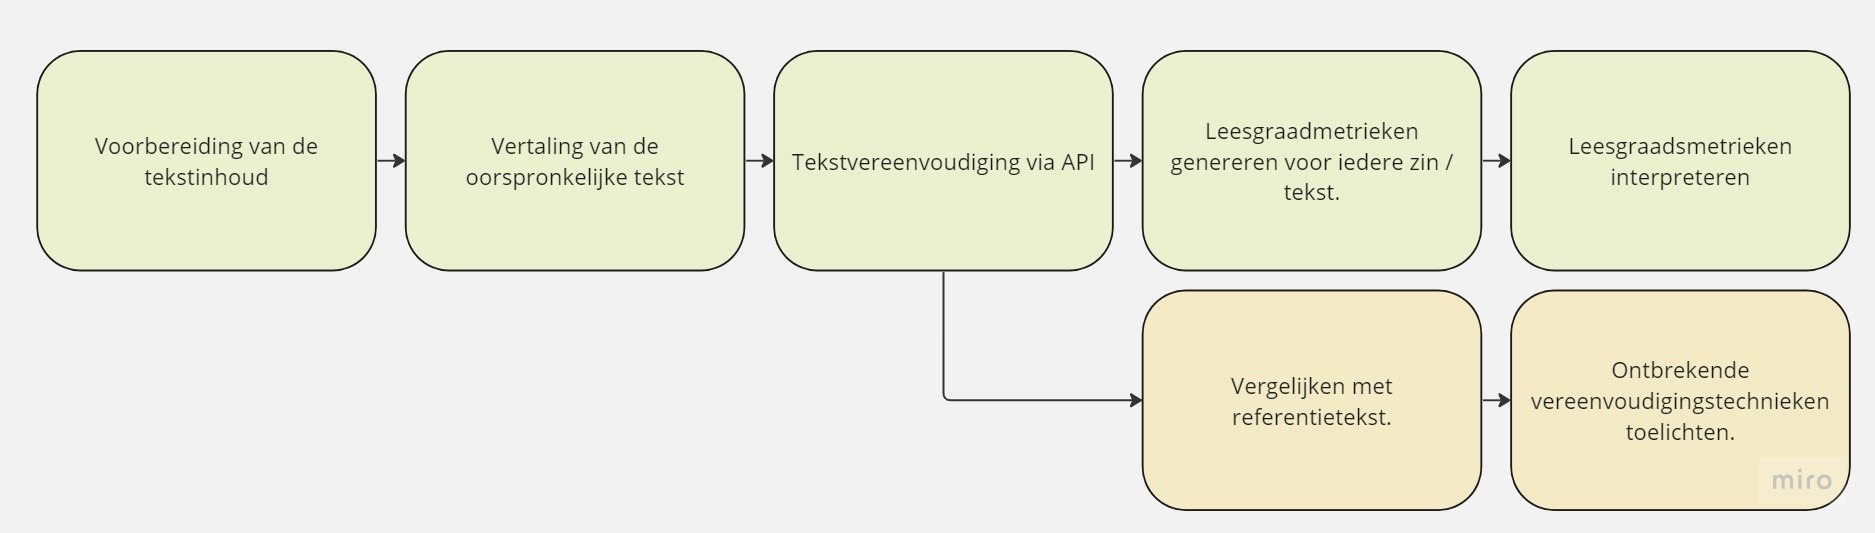
\includegraphics[width=\linewidth]{img/flowchart-vergelijkende-studie.jpg}
\caption{Het gevolgde stappenplan voor de vergelijkende studie.}
\label{img:flowchart-vergelijkende-studie-metrics}
\end{figure}

\medspace

% SCRIPT 1
Eerst volgt er een voorbereiding van de tekstinhoud. Allereerst haalt het script de inhoud van de map met wetenschappelijke artikelen op om deze vervolgens in een tekstbestand te plaatsen, zoals weergegeven in codeblok \ref{code:verg-studie-phase-1}. 

\begin{lstlisting}[language=Python, caption={Script voor fase 1 van de vergelijkende studie.}, label={code:verg-studie-phase-1}]
	def add_newline_after_dot(input_file, output_file):
	with open(input_file, 'r', encoding='utf-8') as file:
	text = file.read()
	text = re.sub(r'\d', '', text)
	modified_text = text.replace('.', '.\n')
	with open(output_file, 'w', encoding='utf-8') as file:
	file.write(modified_text)
	
	folder_path = 'scripts\pdf'
	original_scientific_papers = [f for f in os.listdir(folder_path)]
	
	for paper in original_scientific_papers:
	input_file =  folder_path + '/' + paper
	output_file = folder_path + '/' + 'RE_' + paper
	add_newline_after_dot(input_file, output_file)
\end{lstlisting} 

Vervolgens vertaalt het script de zinnen naar Engels. Het script, verwezen in script \ref{code:verg-studie-phase-2}, doorloopt alle tekstbestanden en vertaalt de tekstinhoud met de \textit{deep\_translator} python-bibliotheek. Zo bekomt het script een csv-bestand met twee kolommen: alle Nederlandstalige en alle vertaalde Engelstalige zinnen van één wetenschappelijk artikel. Als separator gebruikt het csv-bestand een \textit{pipe}-symbool.

\begin{center}
	\begin{lstlisting}[language=Python, caption={Script voor de tweede fase van de vergelijkende studie.}, label={code:verg-studie-phase-2}]
		output_csv = 'results.csv'
		
		def translate_dutch_to_english(dutch_text_file):
		with open(dutch_text_file, 'r', encoding='utf-8') as file:
		dutch_sentences = file.readlines()
		dutch_sentences = [sentence.strip() for sentence in dutch_sentences]
		
		english_sentences = []
		for sentence in dutch_sentences:
		translated = GoogleTranslator(source='nl', target='en').translate(sentence)
		english_sentences.append(translated)
		df = pd.DataFrame({'Dutch': dutch_sentences, 'English': english_sentences})
		df.to_csv(str(dutch_text_file).split('.')[0] + '.csv', index=False)
		
		
		folder_path = 'scripts/pdf/'
		original_scientific_papers = [f for f in os.listdir(folder_path)]
		
		for paper in original_scientific_papers:
		if paper.startswith('RE_') and paper.endswith('.txt'):
		print(f'STARTING {paper}')
		dutch_text_file = folder_path + paper
		translate_dutch_to_english(dutch_text_file)
	\end{lstlisting}
\end{center}


Na de vertaling van de tekstinhoud, stuurt het script API-calls voor iedere zin naar ieder taalmodel. Dit procesde taalmodellen aan om de inhoud van de wetenschappelijke artikelen te vereenvoudigen, weergegeven in listing \ref{code:verg-studie-phase-3}. Allereerst vindt een tokenisatiefase plaats. Daarvoor gebruikt het script de \textit{sentence tokenisation} van Spacy en de verwante \textit{embedding models} weergegeven in tabel \ref{table:wordembeddings-spacy}. Na de tokenisering voert het script API-calls uit. API-calls in de \textit{scientific\_simplify}-functie naar HuggingFace of OpenAI sturen de tekst naar de taalmodellen die de tekst verwerkt. De request naar de HuggingFace API bestaat uit de parameters weergegeven in tabel \ref{table:huggingface-requests-parameters}. Alle HuggingFace taalmodellen vereisen een laadfase. Daarom bevat de \textit{API-call} een extra parameter, namelijk \textit{wait\_for\_model}. Verder past dit script geen extra parameters van de taalmodellen aan. 

\medspace

Zoals aangehaald door \textcite{Gooding2022} kunnen prompt-gebaseerde testen verschillende resultaten krijgen, afhankelijk van de gegeven input. Daarom gebruikt het script drie verschillende prompts, gebaseerd op de MTS-technieken beschreven in tabel \ref{table:manual-simplification}. Tabel \ref{table:tested-prompts} visualiseert de gebruikte prompts voor de testen met het GPT-3 model. 

\medspace

Zowel T1 als T4 gebruiken een \textit{nul-temperature} en een \textit{top-p} waarde van 90\% om vertrouwde antwoorden te krijgen. Daarnaast dient de top-p om een hoge woordfrequentie te verkrijgen, zoals aangegeven in \ref{table:gpt-3-parameters}. Bij T1 zijn deze twee parameters ingebakken in de functie. Nadien verwerken de taalmodellen iedere zin uit de tekst. 

\medspace

Ten slotte beantwoordt de HuggingFace of GPT API in JSON-formaat, bevattende de vereenvoudigde versie van de opgegeven zin. T1, T2 en T3 vereenvoudigen de Engelstalige zinnen, in tegenstelling tot T4 en verwante prompts die de Nederlandstalige zinnen vereenvoudigen. Om een \textit{request failure} door een te lange input te voorkomen, breekt het script de volledige input op per 1000 tokens.


\begin{center}
	\begin{table}[H]
		\begin{tabular}{ | m{7cm} | m{7cm} | } 
			\hline
			\textbf{Taal} & \textbf{Embeddingsmodel} \\
			\hline
			Nederlands & NL Core News Medium\footnote{https://github.com/explosion/spacy-models/releases/tag/nl_core_news_md-3.5.0} \\ 
			\hline
			Engels & EN Core Web Medium\footnote{https://github.com/explosion/spacy-models/releases/tag/en_core_web_md-3.5.0} \\
			\hline
		\end{tabular}
		\caption{Gebruikte SpaCy word-embeddings}
		\label{table:wordembeddings-spacy}
	\end{table}
\end{center}

\begin{center}
	\begin{table}[H]
		\begin{tabular}{ | m{6cm} | m{8cm} | } 
			\hline
			\textbf{Naam parameter} & \textbf{Waarde} \\
			\hline
			Inputs & De oorspronkelijke zin. Enkel bij T1 komt 'simplify:' voor deze zin. \\
			\hline
			Max length & De lengte van de oorspronkelijke zin + 10 tokens. \\
			\hline
			Wait for model & Altijd ingesteld op \textit{True}. \\
			\hline
		\end{tabular}
		\caption{Meegegeven parameters bij HuggingFace-requests}
		\label{table:huggingface-requests-parameters}
	\end{table}
\end{center}

\begin{center}
	\begin{table}[H]
		\begin{tabular}{ | m{2cm} | m{13cm} | } 
			\hline
			\textbf{Naam} & \textbf{Prompt} \\
			\hline
			P1 & Vereenvoudig deze tekst \\
			\hline
			P2 & Vereenvoudig deze tekst voor studenten (16-18 jaar) door moeilijke woorden te vervangen, vakjargon te schrappen, woorden langer dan 18 letters te vervangen, acroniemen voluit te schrijven, een woord slechts eenmaal door een synoniem te vervangen, korte uitleg te geven wanneer dat nodig is, en percentages te vervangen. \\
			\hline
			P3 & Vereenvoudig een tekst door deze op te delen in kortere zinnen van maximaal tien woorden. Verander voornaamwoorden als 'zij', 'hun' of 'hij' in namen. Vervang complexe zinsconstructies en voorzetselzinnen door eenvoudiger alternatieven, maar laat ze ongewijzigd als er geen eenvoudiger optie beschikbaar is. \\
			\hline
		\end{tabular}
		\caption{De GPT-3-prompts die in de vergelijkende studie aan bod komen.}
		\label{table:tested-prompts}
	\end{table}
\end{center}

\begin{center}
	\begin{lstlisting}[language=Python, caption={Script voor de derde fase van de vergelijkende studie}, label={code:verg-studie-phase-3}]		
		folder_path = 'scripts\pdf'
		dutch_spacy_model = "nl_core_news_md"
		english_spacy_model = "en_core_web_sm"
		
		dict = {
			'nl':'nl_core_news_md',
			'en':'en_core_web_sm'
		}
		
		total_df = None
		gt = Translator()
		
		huggingfacemodels = {
			'T1':"https://api-inference.huggingface.co/models/haining/scientific_abstract_simplification",
			'T2': "https://api-inference.huggingface.co/models/sambydlo/bart-large-scientific-lay-summarisation",
			'T3': "https://api-inference.huggingface.co/models/philippelaban/keep_it_simple"
		}
		
		max_length = 2000
		COMPLETIONS_MODEL = "text-davinci-003"
		EMBEDDING_MODEL = "text-embedding-ada-002"
		
		languages = {
			'nl':'nl_core_news_md',
			'en':'en_core_web_md'
		}
		
		class HuggingFaceModels:
			def __init__(self, key=None):
				global huggingface_api_key
				try:
					huggingface_api_key = key
				except:
					huggingface_api_key = 'not_submitted'
				
			def query(self, payload, API_URL):
				headers = {"Authorization": f"Bearer {huggingface_api_key}"}
				response = requests.post(API_URL, headers=headers, json=payload)
				return response.json()
			
			def scientific_simplify(self, text, lm_key):
				try:
					API_URL = huggingfacemodels.get(lm_key)
					translated = GoogleTranslator(source='auto', target='en').translate(str(text))
				
		if lm_key == 'T1':
		result = self.query({"inputs": str('simplify: ' + str(translated)),"parameters": {"max_length": len(sentence)+10},"options":{"wait_for_model":True}}, API_URL)
		else:
		result  = self.query({"inputs": str(translated),"parameters": {"max_length": len(sentence)+10},"options":{"wait_for_model":True}}, API_URL)
		
		
		if 'generated_text' in result[0]:
			translated = GoogleTranslator(source='auto', target='nl').translate(str(result[0]['generated_text']))
			return translated
		elif 'summary_text' in result[0]:
			translated = GoogleTranslator(source='auto', target='nl').translate(str(result[0]['summary_text']))
			return translated
		else:
			return None
		except:
			return text
		
		def get_sentence_length(sentence):
			txt_language = detect(sentence)
			dic_language = languages.get(txt_language)
			nlp = spacy.load(dic_language)
			doc = nlp(sentence)
			return len()	
		
		def tokenize_text(text):
			txt_language = detect(text)
			dic_language = languages.get(txt_language)
			nlp = spacy.load(dic_language)
			doc = nlp(text)
			return doc.sents
			
		
		def process_file(file_path):
			with open(folder_path + '/' + file_path, "r", encoding='utf8') as file:
				text = file.read()
				tokens = tokenize_text(text)
				return tokens
				
		
		hf = HuggingFaceModels(key=os.getenv('huggingface_key'))
		original_scientific_papers = [f for f in os.listdir(folder_path)]
		
		for paper in original_scientific_papers[3:]:
			sentence_tokens = process_file(paper) 
			for sentence in sentence_tokens:
				for model in huggingfacemodels.keys():
					filename = "SIMPLIFIED_"+model+'_'+paper
					with open(filename, 'a', encoding='utf-8') as f:
						output = hf.scientific_simplify(str(sentence), model)
						f.write(str(output)) 	
	\end{lstlisting}
\end{center}

Vervolgens berekent het script leesgraadscores met de \textit{readability} python-bibliotheek. Leesgraadscores dienen, zoals aangegeven in \textcite{Nenkova2004}, als objectieve maatstaf bij deze vergelijkende studie. 

\begin{itemize}
	\item De FRE en FOG zijn relevant, want ze kunnen de moeilijkheidsgraad van een zin of tekst objectief meten.
	\item Het aantal complexe en lange woorden kan wijzen op de gebruikte \textit{substitution generation} van het taalmodel.
	\item Het aantal hulpwerkwoorden en vervoegingen van 'zijn' kan aanduiden op mogelijke passieve stem, wat het onderzoek van \textcite{Ruelas2020} als 'hinderende' zinsyntax vernoemt.
\end{itemize}

Het resultaat van dit script is een \textit{Pandas-dataframe} met alle leesbaarheidsmetrieken uit de \textit{readability}-library. Ten slotte slaat het script de \textit{Pandas-dataframe} op als CSV-bestand.

Listing \ref{code:verg-studie-phase-4} omvat de code om de leesmetrieken per zin bij te kunnen houden. Allereerst laadt het script de twee embeddingsmodellen, weergegeven in tabel \ref{table:wordembeddings-spacy} in. Vervolgens bouwt het script een leeg DataFrame op om de meetresultaten erin op te slaan. Daarna itereert het python-script door alle teruggevonden tekstbestanden om vervolgens deze tekst in te lezen. Voor elke zin wordt geprobeerd om meetwaarden voor leesbaarheid te verkrijgen door gebruik te maken van de functie readability.getmeasures, waarbij de taal 'nl' (Nederlands) wordt gespecificeerd. 


Als het script alle meetwaarden succesvol kan verkrijgen, dan maakt het script een nieuwe rij met de objectieve leesmetrieken. Zo krijgt de dataframe alle leesmetrieken opgesomd in \ref{} . Ten slotte voegt het script alle rijen toe aan de DataFrame. Als er tijdens het meten van de leesbaarheid van een zin een Exception optreedt, dan verwerpt het script die zin voor dat artikel.

\begin{center}
	\begin{table}[H]
		\begin{tabular}{ | m{8cm} | m{7cm} | } 
			\hline
			\textbf{Leesgraadscore} & \textbf{Vereenvoudigingstechniek }\\
			\hline
			FOG & LS en SS \\
			\hline
			FRE & LS en SS \\
			\hline
			Aantal woorden per zinnen & SS \\
			\hline
			Aantal complexe woorden per zin volgens Dale Chall index & LS \\
			\hline
			Aantal lange woorden per zin & LS \\
			\hline
			Aantal gebruikte hulpwerkwoorden & SS \\
			\hline
			Aantal zinnen met een vervoeging van het werkwoord 'zijn' & SS \\
			\hline
		\end{tabular}
		\caption{De objectieve metrieken voor de vergelijking van de vereenvoudigde teksten met de oorspronkelijke tekst en de referentieteksten.}
		\label{table:verg-studie-metrieken}
	\end{table}
\end{center}

\begin{center}
	\begin{lstlisting}[language=Python, caption={Script voor fase 4 van de vergelijkende studie}, label={code:verg-studie-phase-4}]	
		simplified_folder = 'scripts/vereenvoudigde_artikelen'
		original_folder = 'scripts/pdf'
		
		scientific_papers = [original_folder + "/" + f for f in os.listdir(original_folder)] + [simplified_folder + "/" + f for f in os.listdir(simplified_folder)]
		
		languages = {
			'nl':'nl_core_news_md',
			'en':'en_core_web_md'
		}
		
		df = pd.DataFrame()
		
		for paper in scientific_papers:
		with open(paper, 'r', encoding='utf-8') as file:
		text = file.read()
		nlp = spacy.load(languages.get('nl'))
		doc = nlp(text)
		
		for sent in doc.sents:
		try:
		metrics = readability.getmeasures(sent.text, lang='nl')
		row = {
			'Paper': paper.split('/')[2].split('.')[0],
			'Sentence': sent.text,
			'FRE': metrics['readability grades']['FleschReadingEase'],
			'FOG': metrics['readability grades']['GunningFogIndex'],
		}
		
		for key, value in metrics['sentence info'].items():
		row[key] = value
		
		for key, value in metrics['word usage'].items():
		row[key] = value
		
		for key, value in metrics['sentence beginnings'].items():
		row[key] = value
		
		df = df.append(row, ignore_index=True)
		except Exception as e:
		print(e)
		
		df.to_csv('result.csv', index=False)
	\end{lstlisting}
\end{center}

% In de volgende fase komt het visualiseren en interpreteren van de resultaten aan bod, waarbij een \textit{Jupyter-notebook} Matplotlib gebruikt om resultaten te visualiseren.

Tenslotte komen de resultaten van de menselijke beoordeling aan bod. Deze fase van de vergelijkende studie staat stil bij aspecten die leesmetrieken niet kunnen meten, waaronder de normen vermeld in tabel \ref{table:criteria-vergelijkende-studie-human-obv}. De referentietekst dient hier als hulpmiddel om de referentietekst, ofwel het verwachte resultaat, te vergelijken met de vereenvoudigde tekst door een taalmodel. 

\begin{table}[H]
	\begin{tabular}{| m{6cm} | m{6cm} |}
		\hline
		\textbf{Metriek} & \textbf{Vereenvoudigingstechniek} \\ \hline
		Acroniemen behouden & Lexicale vereenvoudiging 	\\ \hline
		Inschatting van de doelgroep & Lexicale vereenvoudiging	\\ \hline
		Behoud van kern- en bijzaken & Lexicale vereenvoudiging \\ \hline
		Schrijven in tabelvorm of als opsomming & Structurele aanpassing \\ \hline
		Passieve zinconstructies herschrijven naar actieve zinconstructies & Syntactische vereenvoudiging \\ \hline
		Bronvermelding behouden &  N.v.t. \\ \hline
		Citeren en parafraseren & N.v.t. \\ \hline
	\end{tabular}
	\caption{Criteria voor menselijke observatie bij de vergelijkende studie.}
	\label{table:criteria-vergelijkende-studie-human-obv}
\end{table}

\section{Prototype voor tekstvereenvoudiging}

Met het Moscow-schema en het geschikte taalmodel voor gepersonaliseerde ATS, kan het onderzoek een volgende stap zetten richting het beantwoorden van de onderzoeksvraag. Deze sectie omschrijft de ontwikkeling van een prototype voor gepersonaliseerde ATS voor scholieren met dyslexie in de derde graad van het middelbaar onderwijs. Daarmee kan de ontwikkeling een antwoord bieden op de volgende deelvraag: 

\begin{itemize}
	\item Hoe kan een intuïtieve en lokale webtoepassing worden ontwikkeld die zowel scholieren met dyslexie als docenten helpt bij het vereenvoudigen van wetenschappelijke artikelen met behoud van semantiek, jargon en zinsstructuren?
\end{itemize}

Voor de ontwikkeling van het prototype volgt het onderzoek de flowchart op figuur \ref{img:general-overview-prototype}. Deze flowchart toont zes algemene fasen. Zo start het onderzoek met een voorbereidende fase waarin het onderzoek de nodige technieken en taalmodellen opsomt. Vervolgens start het onderzoek met de ontwikkeling van de back end en front end. Vervolgens komt de ontwikkeling van het lerarencomponent, gevolgd door de ontwikkeling van het scholierencomponent aan bod. Daarna moet het onderzoek stilstaan bij de opzet van het prototype met behulp van Docker. Ten slotte evalueert het onderzoek het gemaakte prototype aan de hand van het Moscow-schema en de vergelijkende studie. Het lerarencomponent moet wetenschappelijke artikelen kunnen vereenvoudigen, na selectie van gepersonaliseerde ATS-technieken. Daarnaast moet het scholierencomponent ondersteuning bieden. In dit component van het prototype moeten scholieren met dyslexie in \textit{real-time} aanpassingen kunnen maken aan de tekst, alsook ondersteuning krijgen tijdens het begrijpend lezen van een tekst. Gepersonaliseerde opmaakopties moeten over de volledige prototype gelijk blijven.


\begin{sidewaysfigure}
	\begin{figure}[H]
		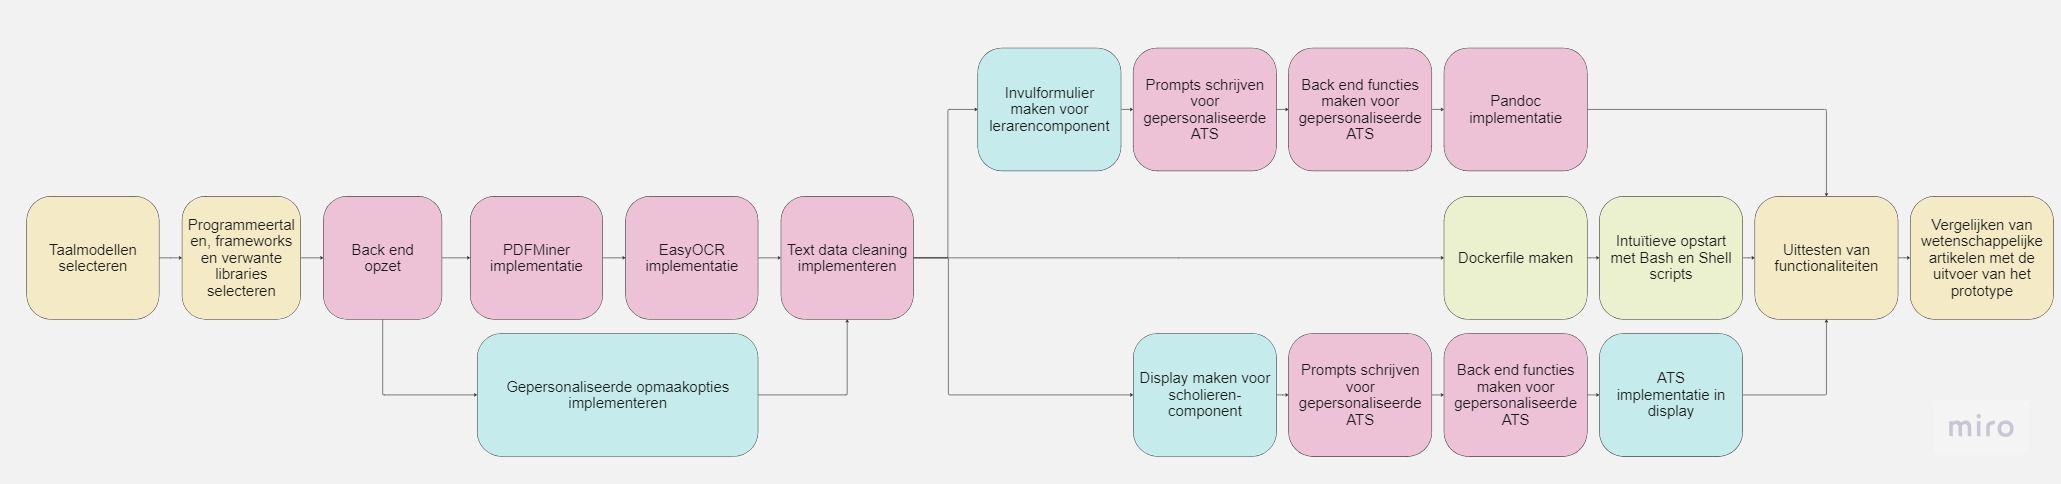
\includegraphics[width=\linewidth]{img/flowchart-general-development.jpg}
		\caption{Algemeen overzicht van de ontwikkeling van het prototype voor ATS van wetenschappelijke artikelen.}
		\label{img:general-overview-prototype}
	\end{figure}
\end{sidewaysfigure}

\subsubsection{Taalmodellen selecteren}

Allereerst bepaalt het onderzoek een taalmodel of meerdere taalmodellen voor gepersonaliseerde ATS, omdat deze keuze later de technologiekeuze kan beïnvloeden. Zo wijst het onderzoek uit dat GPT-3 een geschikt taalmodel is voor gepersonaliseerde ATS. Na de bepaling van het taalmodel bepaalt het onderzoek de technologieën en \textit{frameworks} voor de \textit{back end} en de \textit{front end}. 

\subsubsection{Programmeertalen, frameworks en verwante libraries selecteren}

Omwille van de beschikbaarheid van GPT-3 via API-calls, kunnen python en javascript geschikte keuzes voor dit prototype. Voor een snelle en gratis ontwikkeling gebruikt het prototype \textit{open-source} pakketten. Tabel \ref{table:technologies} toont een breed overzicht van alle gebruikte programmeertalen. Hierop vult tabel \ref{table:python-libraries} aan door een overzicht te geven van alle gebruikte python-libraries.

\begin{center}
	\begin{table}[H]
	\begin{tabular}{ | m{4cm} | m{11cm} | } 
		\hline
		\textbf{Technologie} 	& \textbf{Functionaliteit} \\
		\hline
		Python 					& De back end van het prototype die API-calls en de NLP-functionaliteiten zoals PoS-tagging en lemmatizing verwerkt. \\
		\hline
		JavaScript (JS)				& De toepassing gebruikersvriendelijker maken, personalisatie-opties voor de site doorvoeren en de functies gebouwd in Javascript dienen als alternatief op commandline instructies. \\
		\hline
		HTML en CSS 			& Het visuele uiterlijk van de website aanpassen naargelang de gekozen parameters van de eindgebruiker. \\
		\hline
		Jinja 					& Informatie uit de back end doorgeven aan de front-end.  \\
		\hline
		Docker 					& Lokale uitrol van de webtoepassing. \\
		\hline
		Bash					& Intuïtief script om de webtoepassing op te starten voor Linux en Mac-systemen. \\
		\hline
		Powershell 				& Intuïtief script om de webtoepassing op te starten op Windows-systemen. \\
		\hline
	\end{tabular}
	\caption{Gebruikte programmeertalen in het prototype voor tekstvereenvoudiging.}
	\label{table:technologies}
	\end{table}
\end{center}

\begin{center}
	\begin{table}[H]
	\begin{tabular}{ | m{4cm} | m{11cm} | } 
		\hline
		\textbf{Python-bibliotheek} & \textbf{Functionaliteit} \\
		\hline
		Flask					& Het framework van de webtoepassing. Dit framework combineert front end en back end. \\ 
		\hline
		PDFMiner 				& Tekstinhoud van PDF's extraheren. \\ 
		\hline
		EasyOCR					& PDF-pagina's inscannen als afbeelding in JPG-formaat om vervolgens de tekst te extraheren. \\
		\hline
		NumPy 					& De reshape-functie vereenvoudigt de manier om arrays van zinnen bij elkaar te plaatsen om zo een paragraaf te bekomen. \\
		\hline		
		Spacy 					& PoS-tagging en het lemmatiseren van woorden. \\
		\hline
		OpenAI					& GPT-3 API aanspreken. \\
		\hline
		BeautifulSoup			& HTML-content in het lerarencomponent \textit{parsen} voor een correcte formatting. \\
		\hline
	\end{tabular}
	\caption{Gebruikte Python-libraries en hun respectievelijke functie in het prototype.}
	\label{table:python-libraries}
	\end{table}
\end{center}

\subsubsection{Back end opzet}

Na het kiezen van de taalmodellen en de technologieën en frameworks, start het onderzoek met de front end implementatie. Allereerst voegt het onderzoek een homepagina toe dat als portaal zal dienen voor de leraren- en scholierencomponenten. Allereerst implementeert het onderzoek de nodige personaliseerbare opmaakopties. Zoals aangeraden door \textcite{Galliussi2020}, moeten ontwikkelaars rekening houden met de opmaakopties van de website. Zo maakt het prototype gebruik van alle parameters onderzocht door \textcite{Rello2013a, Rello2013b}. Het instellingenscherm is een HTML-bestand waarin een formulier alle aanpasbare parameters oplijst. Tabel ... toont de opgenomen parameters. De standaardparameters volgen de aangeraden parameters van (...). Het formulier stuurt vervolgens een POST-request naar de back end. De back end verwerkt deze aanvraag en slaat de ontvangen dictionary op als sessievariabele, zoals weergegeven in listing \ref{code:back-end-session-personalized}. 


\begin{lstlisting}[language=python, caption={De back end functie die de aanpassingen uit het formulier opslaat als sessievariabele.}, label={code:back-end-session-personalized}]
PER_SET_SESSION_NAME = 'personalized_settings'

@app.route('/get-settings-user',methods=['POST'])
def return_personal_settings_dict():
	if PER_SET_SESSION_NAME in session:
		return jsonify(session[PER_SET_SESSION_NAME])
	else:
		return jsonify(result='session does not exist')
	
@app.route('/change-settings-user', methods=['POST'])
def change_personal_settings():
	try:
		session[PER_SET_SESSION_NAME] = dict(request.form)
		msg = 'Succesvol aangepast!'
	except Exception as e:
		msg = str(e)
		flash(msg)
	return render_template('settings.html')
\end{lstlisting}

Ten slotte moet de \textit{front end} deze opmaakopties bij iedere wegpagina inladen. Het inladen gebeurt met een \textit{window onload}, zoals weergegeven in listing \ref{code:window-onload-js}. Zo hoeven eindgebruikers deze parameters niet bij iedere webpagina opnieuw aan te passen.

\begin{lstlisting}[language=javascript, caption={De onload-functie die de gepersonaliseerde opmaakopties regelt bij het inladen van een webpagina.}, label={code:window-onload-js}]
window.onload = async function () {
	var url = `http://localhost:5000/get-settings-user`;
	const response = await fetch(url, { method: 'POST' });
	var result = await response.json();
	document.body.style.fontSize        = result.fontSize+'px';
	document.body.style.fontFamily      = result.fontSettings;
	document.body.style.backgroundColor = result.favcolor;
	document.body.style.lineHeight      = result.lineHeight+'cm';
	document.body.style.wordSpacing     = result.wordSpacing+'cm';
	document.body.style.textAlign       = result.textAlign;
}
\end{lstlisting}

Naast de gepersonaliseerde opmaakopties, moet het prototype ook over een systeem beschikken dat wetenschappelijke manieren kan opladen en inlezen. Zo biedt het prototype twee manieren aan om wetenschappelijke artikelen in te laten: via \textit{plaintext} of via een PDF-bestand. Niet alle \textit{PDF extractors} zijn foutbestendig, want zoals eerder opgemerkt in de \ref{sec:requirementsanalyse} kunnen \textit{PDF extractors} ook tekst verliezen tijdens dit proces. Als valnet biedt het prototype een OCR-optie aan. Deze functionaliteit omvat de ontwikkeling van functionaliteiten aan de front-end en aan de back end.

\medspace

De \textit{front end} kent enkel de toevoeging van een checkbox en twee \textit{input-tags}, namelijk een \textit{file-input} en een \textit{textarea-input}. De \textit{file-input} geeft de binaries van het PDF-bestand mee van de front-end naar de back end die het PDF-bestand tijdelijk \textit{in-memory} opslaat. Daarnaast krijgt de back end de keuze van de gebruiker tussen normale en OCR-upload mee als boolean, waarbij 1 gelijk staat aan een OCR-afhandeling. Ten slotte gebruikt het formulier een POST-request om alle meegekregen informatie door te sturen naar de back end. Na het ontvangen van de request van de front-end, handelt de Flask back end het bestand verder af zoals aangewezen in listing \ref{code:inlezen-wetenschappelijk-artikel-front-end-back-end}. Eerst controleert de \textit{back end} het type invoer. Vervolgens spreekt de Flask back end de Reader-klasse aan die de tekst formatteert tot een bruikbaar formaat voor de webtoepassing. Daarna gebruikt de Reader-klasse één van twee mogelijke technieken. 

\begin{lstlisting}[language=Python, caption={Koppeling tussen front-end en back-end voor het inlezen van een wetenschappelijk artikel}, label={code:inlezen-wetenschappelijk-artikel-front-end-back-end}]
def setup_scholars_teachers(request):
	settings = request.form
	if 'fullText' in request.form:
		text = request.form['fullText']
		langs = detect_langs(text)
		reader = Reader()
		dict_text = reader.get_full_text_site(text)                
	elif 'pdf' in request.files:
		if 'advanced' not in settings:
			pdf = request.files['pdf']
			pdf_data = BytesIO(pdf.read())
			all_pages = extract_pages(pdf_data,page_numbers=None,maxpages=999)
			langs = detect_langs(str(all_pages))
			reader = Reader()
			full_text = reader.get_full_text_dict(all_pages)
			dict_text = reader.get_full_text_site(full_text)
		else:
			pdf = request.files['pdf']
			pdf_data = pdf.read()
			pages = convert_from_bytes(pdf_data)
			reader = Reader()
			img_text = reader.get_full_text_from_image(pages)
			langs = detect_langs(img_text)
			dict_text = reader.get_full_text_site(img_text)                            
			return dict_text, langs, 'voorbeeldtitel', 'voorbeeldonderwerp'
			
@app.route('/for-scholars', methods=['GET','POST'])
def teaching_tool():
	try:
		dict_text, langs, title, subject = setup_scholars_teachers(request)
		return render_template('for-scholars.html', pdf=dict_text, lang=langs, title=title, subject=subject)
	except Exception as e:
		return render_template('error.html',error=str(e))
	
@app.route('/for-teachers', methods=['GET','POST'])
def analysing_choosing_for_teachers():
	try:
		dict_text, langs, title, subject = setup_scholars_teachers(request)
		return render_template('for-teachers.html', pdf=dict_text, lang=langs, title=title, subject=subject)
	except Exception as e:
		return render_template('error.html',error=str(e))
\end{lstlisting}

\subsubsection{PDFMiner implementatie}

Bij een gewone PDF-extractie gebruikt de Reader-klasse PDFMiner met de functie in listing \ref{code:inlezen-van-pdf}. Deze functie itereert doorheen alle PDF-pagina's van een meegekregen \textit{in-memory} pdf. Nadien extraheert de functie alle tekst op een pagina. Nadien concateneert deze functie alle opgehaalde tekst van één pagina aan een lege string. De functie herhaalt dit proces tot het script geen pagina's meer kan inlezen. Het resultaat van deze functie is een string-object met alle geëxtraheerde tekst uit een pdf.

\begin{lstlisting}[language=Python, caption={Een PDF inlezen met PDFMiner}, label={code:inlezen-van-pdf}]
	def get_full_text_from_pdf(self, all_pages):
		total = ""
		for page_layout in all_pages:
			for element in page_layout:
				if isinstance(element, LTTextContainer):
				for text_line in element:
					total += text_line.get_text()
					return total
\end{lstlisting}

\subsubsection{EasyOCR implementatie}

PDFMiner kan tekst missen bij de pdf-extractie. Daarom voorziet het prototype een valnet met een OCR-techniek. De Python-bibliotheek EasyOCR voorziet een eenduidige en ontwikkelaarsvriendelijke manier om tekst uit pdf's te extraheren met OCR-technieken. Zo itereert EasyOCR over alle pagina's in een PDF en slaat iedere pagina op als een JPG-bestand. Vervolgens leest EasyOCR de tekst op iedere pagina in en houdt dit bij tot het einde van het script. Na het inlezen van de tekst, verwijdert het script de aangemaakte afbeeldingen om zo geheugenruimte te besparen. Net zoals bij de eerste methode, resulteert deze methode in een string-object met alle tekst uit de PDF. De uitgewerkte code staat uitgeschreven in listing \ref{code:reader-ocr}

\begin{lstlisting}[language=Python, caption={Een PDF inlezen met OCR}, label={code:reader-ocr}]
	def get_full_text_from_image(self, all_pages):
		img_files = []
		num_pages = 0
		for i, page in enumerate(all_pages):
			file = f'page_{num_pages}.jpg'
			page.save(file, 'JPEG')
			img_files.append(file)
			num_pages += 1
		
		full_text = []
		reader = easyocr.Reader(['nl'])
		for f in img_files:
			result = reader.readtext(f, detail=0)
			full_text.append(" ".join(result))
			os.remove(f)
		return " ".join(full_text)
\end{lstlisting}

\subsubsection{Geëxtraheerde inhoud formatteren naar een webpagina.}

Na het extraheren van de tekstinhoud, komt een formatteerfase aan bod. Hier vormt het systeem de tekst om naar het gewenste formaat voor de front end. Allereerst transformeert de back end de string van geëxtraheerde tekst naar \textit{arrays} van zinnen met Spacy \textit{word embeddings} en \textit{sentence embeddings}. Deze functie staat beschreven in listing \ref{code:reader-formatting}. Het prototype bundelt vijf zinnen met de \textit{reshape-functie} van Numpy. Eindgebruikers kunnen deze parameter aanpassen in het instellingenscherm. Om de PoS-tag bij het respectievelijke woord bij te houden, gebruikt het prototype een \textit{key-value pair} datastructuur. Zo verwijst de sleutel naar een woord in een zin en de waarde verwijst naar de PoS-tag. Het prototype houdt rekening met enkel Nederlandstalige en Engelstalige wetenschappelijke artikelen. Daarom laadt het prototype hoogstens twee embeddingsmodellen op. Deze embeddingsmodellen staan vermeld in tabel \ref{table:wordembeddings-spacy}. Het prototype vermijdt hardcoderen. Daarom maakt het gebruik van een \textit{dictionary} die de naam van deze embeddingsmodellen bijhoudt. Het prototype gebruikt Engels als standaardtaal, als de back end de taal niet kan herkennen of als de taal niet in de lijst van de dictionary staat. 

\begin{lstlisting}[language=Python, caption={Het formatteren van de tekst naar een formaat voor de website.}, label={code:reader-formatting}]
	def get_full_text_site(self, full_text):
	try:
	lang = detect(full_text)
	except:
	lang = 'en'
	
	if lang in dict:
	nlp = spacy.load(dict.get(lang))
	else:
	nlp = spacy.load(dict.get('en'))
	
	full_text = str(full_text).replace('\n', ' ')
	
	doc = nlp(full_text)
	sentences = []
	for sentence in doc.sents:
	sentences.append(sentence)
	
	pad_size = SENTENCES_PER_PARAGRAPH - (len(sentences) % SENTENCES_PER_PARAGRAPH)
	padded_a = np.pad(sentences, (0, pad_size), mode='empty')
	paragraphs = padded_a.reshape(-1, SENTENCES_PER_PARAGRAPH)
	
	text_w_pos = []
	for paragraph in paragraphs:
	paragraph_w_pos = []
	try:
	for sentence in paragraph:
	dict_sentence = {}
	for token in sentence:
	dict_sentence[token.text] = str(token.pos_).lower()
	paragraph_w_pos.append(dict_sentence)    
	text_w_pos.append(paragraph_w_pos)
	except:
	pass
	return text_w_pos
\end{lstlisting}

Zowel het leraren- als het scholierencomponent passen deze dynamische HTML-structuur in hun weergave toe. Zo zijn er vier verschillende klassen die aan span-tags in deze weergave worden toegekend. Door middel van een Jinja-iteratie, krijgt iedere \textit{span-tag} een specifieke klasse afhankelijk van de key of iteratie. Deze iteratie toont listing \ref{code:html-span-tags} voor. Zo is er een overkoepelende span-tag \textit{sentence}, alsook voor ieder woord in een zin hoort er een span-tag met \textit{nouns}, \textit{adjectives} of \textit{verbs}. Andere woorden, zoals conjuncties, behoren tot de klasse \textit{other}. Na het extraheren van de tekstinhoud van een wetenschappelijk artikel, komt de ontwikkeling van het leraren- en scholierencomponent aan bod. Hoewel ontwikkelaars de ontwikkeling van beide componenten parallel kunnen laten lopen, start het onderzoek met de werkwijze voor de ontwikkeling van het lerarencomponent.

\begin{lstlisting}[language=html, caption={Het doorlopen van de PDF-tekst op de webpagina en het toekennen van de span-tags.}, label={code:html-span-tags}]

	<p class="left-side">
		
		<span class="sentence">
			
			
			<span class={{sentence[word]}}>{{word}}</span>
			
			
		</span>
	
	</p>

\end{lstlisting}


\subsubsection{Invulformulier maken voor het lerarencomponent.}

Zo kunnen leerkrachten beschikken over een tool waarin zij de geëxtraheerde tekstinhoud kunnen manipuleren, om vervolgens opties voor gepersonaliseerde ATS te selecteren. Figuur \ref{img:proto-lerarencomponent} toont een mogelijke weergave van deze HTML-pagina. Leerkrachten moeten in dit lerarencomponent kunnen beschikken over de functionaliteiten weergegeven in tabel \ref{table:functionaliteiten-leerkrachten}. Tabel \ref{table:criteria-requirementsanalysis} reikt de benodigde opties voor gepersonaliseerde ATS aan. Het prototype gebruikt deze criteria als opties om de prompts dynamisch op te bouwen.

\begin{center}
	\begin{table}[H]
		\begin{tabular}{ | m{7cm} | m{8cm} | } 
			\hline
			\textbf{Functionaliteit} & Gebruikte JS of python-techniek \\
			\hline
			Specifieke prompt meegeven per paragraaf & Naast een optie om voor het hele document één prompt te gebruiken, voegt het prototype ook een optie toe om. Hiervoor past de web-inhoud een key-value structuur toe. \\
			\hline
			Opties voor gepersonaliseerde ATS aanreiken. & Met behulp van een HTML-formulier kunnen leerkrachten opties aanvinken waaraan de vereenvoudigde tekst moet voldoen. \\
			\hline
			Werkwoorden, bijvoeglijke en zelfstandige naamwoorden markeren & Front-end aanpassing met \textit{eventlistener}. De tekstkleur van het aangeduide type woorden verandert naar het gekozen kleur. \\
			\hline
			Zinnen verwijderen & \textit{Front-end} filter aangesproken door een \textit{eventlistener}. \\
			\hline
			Woord toevoegen aan de woordenlijst & Een \textit{eventlistener} handelt de functionaliteit af door de woorden en hun zin van voorkomen tijdelijk op te slaan in een storage. Het formulier houdt dit bij en geeft het vervolgens mee bij het indienen. Deze woorden en hun respectievelijke zin van voorkomen dienen om de woordenlijst op te vullen in het gegenereerde PDF of Word-bestand. \\ 
			\hline
			Sleutel en sessieherkenning & . \\
			\hline 
		\end{tabular}
	\caption{Alle beschikbare functionaliteiten in }
	\label{table:functionaliteiten-leerkrachten}
	\end{table}
\end{center}

\subsubsection{Prompts schrijven voor gepersonaliseerde ATS in het lerarencomponent}

Het onderzoek stelt de prompts op volgens de richtlijnen beschreven in tabel \ref{table:techniques-for-good-prompts}. Daarnaast past het Intent- en Contextualization prompts toe zoals aangeraden door \textcite{White2023}. Tabel \ref{table:prompts-lerarencomponent} geeft een overzicht van alle opgestelde prompts die het prototype gebruikt in het lerarencomponent. Daarnaast gebruikt iedere API-call de parameters omschreven in tabel \ref{table:gpt-3-parameters-lerarencomponent}.

\begin{center}
	
\end{center}
\begin{table}[H]
	\begin{tabular}{ | m{5cm} | m{10cm} |}
		\hline
		\textbf{Functionaliteit} & \textbf{Prompt} \\ \hline
		Synoniem opzoeken & Geef een eenvoudiger synoniem voor '{woord}'. Context {context}. \\ \hline
		Definitie opzoeken & Geef een eenvoudige definitie voor '{woord}'. Context {context}.\\ \hline
		Zin vereenvoudigen & \\ \hline
		Gepersonaliseerde ATS & \\ \hline
		Gepersonaliseerde ATS als opsomming & Herschrijf dit als een lijst van vereenvoudigde zinnen met (gepersonaliseerde opties) :return: een lijst van vereenvoudigde zinnen gesplitst door een '|' teken /// {context}\\ \hline
	\end{tabular}
	\caption{Tabel met de gebruikte prompts voor het lerarencomponent.}
	\label{table:prompts-lerarencomponent}
\end{table}

\begin{center}
	\begin{table}[H]
		\begin{tabular}{| m{5cm}| m{10cm} |}
			\hline
			Parameter & Gebruikte waarde \\ \hline
			Prompt & Zie tabel \ref{table:prompts-lerarencomponent} \\ \hline
			Temperature & 0 \\ \hline
			Max tokens & De lengte van het woord vermeerdert met tien tokens als het over het opzoeken van een definitie of synoniem gaat. \\ 
			& Of de lengte van de zin vermeerdert met twintig tokens indien het over vereenvoudiging van een zin gaat. \\
			\hline
			Model & Da Vinci 3 \\ \hline
			Top-p & 90\% \\ \hline
			Stream & False \\ \hline
		\end{tabular}
		\caption{Gebruikte parameters om de definitie van een woord te genereren met GPT-3.}
		\label{table:gpt-3-parameters-lerarencomponent}
	\end{table}
\end{center}


\subsubsection{Back end functies maken voor gepersonaliseerde ATS}

Leraren kunnen handmatig zinnen uit de tekst verwijderen. Hiervoor gebruikt de \textit{front end} een \textit{eventlistener} die de aangeklikte span-tag van klasse 'sentence' uit het HTML-document verwijdert. Naast zinnen verwijderen kunnen leraren ook woorden aan een woordenlijst toevoegen. Hiervoor gebruikt de front-end een JS-script met een \textit{eventlistener} die een woord en de toebehorende zin toevoegt aan een \textit{textarea}. Deze \textit{textarea} gebruikt een \textit{pipe}-symbool als separator om nadien de text te splitsen en een array te bekomen. Om de leerkracht opties aan te reiken voor gepersonaliseerde ATS, bevat het HTML-document een formulier met keuzes aan. Dit formulier bevat alle nodige MTS-technieken uit tabel \ref{table:criteria-requirementsanalysis}. Na een POST-request krijgt de back end deze parameters die het systeem nadien verwerkt in de prompt voor het GPT-3 taalmodel, zoals aangewezen in listing \ref{listing:gpt-class}. Leraren kunnen ook het uitvoerbestand personaliseren met lettertypes, gekozen regeleinde, woord-spatiëring en de marge van het document. Nadat de back end de inhoud van dit formulier ontvangt, neemt de GPT-klasse de aanvraag over. Deze klasse verwerkt drie functionaliteiten, namelijk definities en synoniemen opzoeken en gepersonaliseerde ATS.

\medspace

Allereerst dient de \textit{look-up} functie om de definitie van een woord te achterhalen. Zo beschrijft listing \ref{listing:gpt-look-up-word} de functie om met GPT-3 een eenvoudige definitie van een woord te genereren. Om de uitvoer zo waarschijnlijk mogelijk te maken, gebruikt de GPT-3 API-call een \textit{nultemperature}. Daarna haalt het script het verkregen antwoord uit de JSON-response om deze vervolgens tijdelijk bij te houden in een dictionary.

\begin{lstlisting}[language=Python, caption={Een functie om met GPT-3 een vereenvoudigde definitie voor een woord te genereren.}, label={listing:gpt-look-up-word}]
def look_up_word_gpt(self, word, context):
	try:
	prompt = f"""
	Give a simple Dutch explanation in one sentence for this word in the given context. Give the PoS-tag and Dutch definition: '{word}'
	context: {context}
	format: PoS-tag | definition
	"""

	result = openai.Completion.create(
	prompt=prompt,
	temperature=0,
	max_tokens=50,
	model=COMPLETIONS_MODEL,
	top_p=0.9,
	stream=False
	)["choices"][0]["text"].strip(" \n")    
	return result, word, prompt	
	except Exception as e:
	return 'error', str(e), str(e)
\end{lstlisting}

Vervolgens gebruikt de back end het GPT-3 model om een synoniem op te zoeken. Hiervoor spreekt de API de functie \textit{give-synonym} aan, verwezen in listing \ref{listing:gpt-class}.

\begin{lstlisting}[language=Python, caption={Een synoniem genereren of ophalen met GPT-3.}, label={listing:gpt-give-synonym}]
	""" @returns prompt, result from gpt """
	def give_synonym(self, word, context):
	try:
	prompt = f"""
	Give a Dutch synonym for '{word}'. If there is no Dutch synonym available, explain it between curly brackets.
	context:
	{context}
	"""
	
	result = openai.Completion.create(
	prompt=prompt,
	temperature=0,
	max_tokens=10,
	model=COMPLETIONS_MODEL,
	top_p=0.9,
	stream=False
	)["choices"][0]["text"].strip(" \n")    
	return result, word, prompt
	except Exception as e:
	return 'Open AI outage of problemen', str(e)
\end{lstlisting}
	
Daarna komt de vereenvoudiging van zinnen aan bod. Listing \ref{listing:gpt-personalised-simplify} bevat de code die deze API-call afhandelt. Echter moet het script rekening houden met twee aspecten. Allereerst kan de leerkracht kiezen voor een opsomming van de tekst. Daarnaast moet de inputlengte overeenstemmen met de beperkingen van de GPT-3 API. Wetenschappelijke artikelen zijn bijna altijd langer dan de mogelijk inputlengte. Daarom splitst het prototype de oorspronkelijke tekst op per 1000 tokens, zodat de inputprompt over marge beschikt en daardoor alle nodige gepersonaliseerde ATS-opties mee kan geven. Bij deze splitsing houdt het script rekening met de volledigheid van een zin. 
	
\begin{lstlisting}[language=Python, caption={Een zin gepersonaliseerd vereenvoudigen met GPT-3.}, label={listing:gpt-personalised-simplify}]
def personalised_simplify(self, sentence, personalisation):
	if 'summary' in personalisation:
		prompt = f"""
		Simplify the sentences in the given text and {", ".join(personalisation)}
		:return: A list of simplified sentences divided by a '|' sign
		///
		{sentence}
		"""
	else:
		prompt = f"""
		Explain this in own Dutch words and {", ".join(personalisation)}
		///
		{sentence}
		"""
	
	try:
		result = openai.Completion.create(
		prompt=prompt,
		temperature=0,
		max_tokens=len(prompt),
		model=COMPLETIONS_MODEL,
		top_p=0.9,
		stream=False
		)["choices"][0]["text"].strip(" \n")
		
		if 'summary' in personalisation:
			result = result.split('|')
		else:
			result = [result]
			
			return result, prompt
	except Exception as e:
		return str(e), prompt 
\end{lstlisting}


\subsubsection{Pandoc implementatie}

Ten slotte giet het script de \textit{plain-text} van vereenvoudigde tekstinhoud en de woordenlijsten in een PDF- of DOCX-bestand. Zo maakt de Creator-klasse PDF's en docx-documenten volgens de meegegeven opmaakopties en maakt gebruik van Pandoc via python.  Pandoc gebruikt een tweestapsbeweging, waarbij het eerst \textit{plain-text} naar een markdownformaat omzet en vervolgens het Markdown-bestand naar een PDF of Word-document converteert. Daarvoor is een YAML-header nodig die de elementen, beschreven in tabel \ref{table:personalized-pdf-word-document-with-pandoc}, moet bevatten. Het script in listing \ref{} voegt de meegekregen instellingen toe aan de YAML-header. 

\begin{table}[H]
	\begin{tabular}{ | m{5cm}| m{10cm} | }
		\hline
		\textbf{Label in YAML-header} & \textbf{Voorbeeldwaarde} \\ \hline
		Title & Surveillance met artificiële intelligentie. \\ \hline
		Mainfont & Arial \\ \hline 
		Titlefont & Arial Black \\ \hline
		Date & 14-06-2023 \\ \hline 
		Document & Article \\ \hline
		Margin & 3cm \\ \hline
		Word-spacing & 0.3cm \\ \hline 
		Lineheight & singleheight \\ \hline
	\end{tabular}
	\caption{Benodigde labels voor een gepersonaliseerd document met Pandoc.}
	\label{table:personalized-pdf-word-document-with-pandoc}
\end{table}

Listing \ref{code:yaml-header-function} bouwt de YAML-header op voor het markdownbestand. Deze header is volledig parameteriseerbaar.

\begin{lstlisting}[language=Python, caption={Writer-klasse omvattende de code om dynamische PDF- en Word-documenten te genereren.}, label={code:yaml-header-function}]
	markdown_file = "saved_files/file.md"
	DATE_NOW = str(date.today())
	
	class Creator():
	def create_header(self, title, margin, fontsize, chosen_font, chosen_title_font, word_spacing, type_spacing):
		with open(markdown_file, 'w', encoding='utf-8') as f:
			f.write("---\n")
			f.write(f"title: {title}\n") 
			f.write(f"mainfont: {chosen_font}.ttf\n")
			f.write(f"titlefont: {chosen_title_font}.ttf\n")
			f.write(f'date: {DATE_NOW}\n')
			f.write(f'document: article\n')
			f.write(f'geometry: margin={margin}cm\n')
			f.write(f'fontsize: {fontsize}pt\n')
			f.write('header-includes:\n')
			f.write(f'- \spaceskip={word_spacing}cm\n')
			f.write(f'- \\usepackage{{setspace}}\n')
			f.write(f'- \{type_spacing}\n')
			f.write("---\n")
\end{lstlisting}

Om de woordenlijst aan het markdown-bestand toe te voegen, bouwt het script eerst een \textit{dictionary}-structuur op met de positie van het woord als key en als values de woord, de PoS-tag en de opgehaalde gepersonaliseerde betekenis. Het prototype moet rekening houden met homoniemen en daarom kan de key hier niet het woord zijn. Bij een lege woordenlijst komen deze bewerkingen niet aan bod. 

\begin{lstlisting}[language=Python, caption={Een woordenlijst genereren met de Writer-klasse.}, label={code:writer-glossary-klasse}]
def generate\_glossary(self, list):
with open(markdown_file, 'a', encoding='utf-8') as f:
f.write("---\n")
f.write("# Woordenlijst\n")
f.write("| Woord | Soort | Definitie |\n")
f.write("| --- | --- | --- |\n")
for word in list.keys(): 
f.write(f"| {word} | {list[word]['type']} | {list[word]['definition']} |\n")
\end{lstlisting}

Deze functie vult het markdown-bestand met de vereenvoudigde tekst, gesplitst door de titels die de leerkracht heeft gekozen. Het script slaat de vereenvoudigde tekst nadien op in een \textit{dictionary}-structuur. Vervolgens print het script de vereenvoudigde tekst uit naar het markdown-bestand door alle titels van de \textit{dictionary}-structuur te doorlopen. Een titel uitprinten in markdown syntax moet voorafgaan aan twee \textit{hashtags}, gevolgd door een \textit{breakline}. 

\begin{lstlisting}[language=Python, caption={Een doorlopende tekst toevoegen aan het markdownbestand met de Writer-klasse.}, label={code:writer-doorlopende-klasse}]
def generate_simplification(self, full_text):
with open(markdown_file,'a', encoding="utf-8", errors="surrogateescape") as f:
for key in full_text.keys():
title = str(key).replace('\n',' ')
text = full_text[key]
f.write('\n\n')
f.write(f'## {title}')
f.write('\n\n')
f.write(" ".join(text))
f.write('\n\n')
\end{lstlisting}

Indien de leerkracht een opsomming wenste, dan dient de titel nog steeds al separator, maar het script print de zinnen uit als opsomming conform aan de Markdown-syntax. Na de titel print het script de vereenvoudigde tekst per paragraaf uit. Bij een opsomming gaat een asterisk-symbool vooraf. Vervolgens converteert Pandoc het Markdown-bestand naar een PDF-bestand gebouwd met de XeLateX engine of een Word-bestand met de meegekregen binaries. 

\begin{lstlisting}[language=Python, caption={Een opsomming toevoegen aan het markdownbestand met de Writer-klasse.}, label={code:writer-summation-klasse}]
def generate_simplification_w_summation(self, full_text):
with open(markdown_file,'a', encoding="utf-8", errors="surrogateescape") as f:
for key in full_text.keys():
title = str(key).replace('\n',' ')
text = full_text[key][0].split('|')
f.write('\n\n')
f.write(f'## {title}')
for sentence in text:    
f.write('\n\n')
f.write(f'* {sentence}')
f.write('\n\n')
\end{lstlisting}

Tenslotte maakt het script de pdf en docx-bestanden van de vereenvoudigde teksten. De functie verwezen in listing \ref{code:writer-create-pdf} gebruikt alle bovenstaande (nodige) functies. Daarna genereert Pandoc de pdf en docx-bestanden. Nadien zal de functie deze twee bestanden comprimeren tot één zip-bestand. Hoewel Flask maar één bestand kan teruggeven, comprimeert het script met de \textit{zipfile} bibliotheek deze twee bestanden tot één bestand. Zo krijgt de eindgebruiker alsnog zowel het docx als het pdf-document. 

\begin{lstlisting}[language=Python, caption={Een zip-bestand aanmaken met daarin een docx en pdf bestand van de vereenvoudigde tekst.}, label={code:writer-create-pdf}]
def create_pdf(self, title, margin, list, full_text, fonts, word_spacing, type_spacing, summation):
if title is not None:
self.create_header(title=title, margin=margin, fontsize=14, chosen_font=fonts[0], chosen_title_font=fonts[1], word_spacing=word_spacing, type_spacing=type_spacing)
else:
self.create_header(title='Vereenvoudigde tekst', margin=0.5, fontsize=14, chosen_font=fonts[0], chosen_title_font=fonts[1], word_spacing=word_spacing, type_spacing=type_spacing)

"""GLOSSARY"""
if len(list) != 0:
self.generate_glossary(list=list)

"""SUMMARY"""
if summation:
self.generate_summary_w_summation(full_text=full_text)
else:
self.generate_summary(full_text=full_text)

"""FILE_CREATION"""
pypandoc.convert_file(source_file=markdown_file, to='docx', outputfile=docx_file,   extra_args=["-M2GB", "+RTS", "-K64m", "-RTS"])
pypandoc.convert_file(source_file=markdown_file, to='pdf',  outputfile=pdf_file,    extra_args=['--pdf-engine=xelatex'])
with zipfile.ZipFile(zip_filename, 'w') as myzip:
myzip.write(pdf_file)
myzip.write(docx_file)
\end{lstlisting}

De functionaliteiten van het lerarencomponent stoppen hier. Vervolgens komt het scholierencomponent aan bod, waarbij de nadruk ligt op het ontwikkelen van een ondersteunende tool.

\subsection{De ontwikkeling van het scholierencomponent.}

Tabel \ref{table:beschikbare-functionaliteiten-scholierencomponent} geeft een overzicht van alle functionaliteiten die in het scholierencomponent moeten zitten.

\begin{table}
	\begin{tabular}{| m{10cm} | m{5cm} |}
		\hline
		\textbf{Functionaliteit} & \textbf{JS/GPT-3} \\ \hline
		Zinnen verwijderen & Enkel JS \\ \hline
		Zinnen vereenvoudigen met gepersonaliseerde keuzes & GPT-3 en JS \\ \hline
		Zinnen vereenvoudigen met prompt & GPT-3 en JS \\ \hline
		Woord aan woordenlijst toevoegen & GPT-3 en JS \\ \hline
		Woorden (werkwoorden, bijvoeglijke en zelfstandige naamwoorden) markeren & JS \\ \hline
	\end{tabular}
	\caption{Beschikbare functionaliteiten in het scholierencomponent.}
	\label{table:beschikbare-functionaliteiten-scholierencomponent}
\end{table}

\subsubsection{Display maken voor scholierencomponent}

Net zoals bij het lerarencomponent, moet het prototype een oorspronkelijke weergave van het wetenschappelijk artikel kunnen tonen. Het onderzoek baseert de lay-out op dat van de erkende softwarepakketten, alsook de uitgeteste chatbots. 

\subsubsection{Prompts schrijven voor gepersonaliseerde ATS}

De prompts in tabel \ref{table:prompts-lerarencomponent} kan het scholierencomponent overnemen van het lerarencomponent. Aanvullend op deze prompts kunnen scholieren ook zelf een prompt schrijven.

\subsubsection{Back end functies schrijven voor gepersonaliseerde ATS}

Om zinnen in de doorlopende tekst te verwijderen, moet de front end over de nodige span-tags beschikken. Bij het inlezen van de PDF voert de back end dit al uit, zoals verwezen in listing \ref{code:reader-formatting}. Daarom hoeft het onderzoek geen nieuwe functie in de back end te schrijven. Vervolgens moet de back end over een functie beschikken om een zin te vereenvoudigen. Het lerarencomponent gebruikt al dergelijk functie. Daarmee hergebruikt de \textit{back end} de functie in listing \ref{listing:gpt-personalised-simplify}. 

\medspace

Zinnen baseren op een zelfgemaakte prompt moet de \textit{back end} echter wel toevoegen. Zo gebruikt de back end de functie in listing \ref{code:custom-prompt} om een \textit{custom prompt} te verwerken. Deze functie stuurt de oorspronkelijke prompt, samen met de context, door naar de GPT-3 API.

\begin{lstlisting}[language=python, caption={Een API-call sturen naar GPT-3 met een custom prompt.}, label={code:custom-prompt}]
def personalised_simplify_w_prompt(self, sentences, personalisation):
	try:
		result = openai.Completion.create(
			prompt=personalisation,
			temperature=0,
			max_tokens=len(personalisation)+len(sentences),
			model=COMPLETIONS_MODEL,
			top_p=0.9,
			stream=False
		)["choices"][0]["text"].strip(" \n")
		return result, personalisation
	except Exception as e:
		return str(e), personalisation
\end{lstlisting}

% 4.

Vervolgens heeft de back end als een functie die een woord opzoekt met GPT-3. Deze functie staat beschreven in listing \ref{listing:gpt-look-up-word} en de back end kan deze functie zonder problemen hergebruiken. Ten slotte hoeft de \textit{back end} geen nieuwe functie te krijgen om woordmarkering af te handelen.

\subsubsection{Front end implementatie voor ATS functionaliteiten}

% 1.

Allereerst kan de \textit{front end} zonder hulp van de \textit{back end} zinnen met JS verwijderen. Alle woorden in een zin bundelt de front end in een span-tag van de klasse 'sentence'. Als de gebruiker dergelijk span-tag aanklikt, dan verwijdert de \textit{front end} de gekozen span-tag.

% 2.

Eerst slaat JS de gemarkeerde tekst en meegekregen ATS-opties op en geeft deze door aan de back end met een API-call. Vervolgens verwerkt de back end deze aanvraag door een nieuwe aanvraag te sturen naar GPT-3, met daarin een prompt die de tekst en de gekozen ATS-technieken bevat. De prompt specifieert het formaat waaraan de uitvoer van het taalmodel moet voldoen.  Als de tekst doorlopend is, dan verwerkt JS dit resultaat als een p-tag.  Als het taalmodel een opsomming moest genereren, dan zal de front-end alle zinnen doorlopen en uitprinten tussen twee li-tags.

% 3.

Listing \ref{code:frontend-add-word-to-glossary} toont de aanpak om via de front end een woord, pos-tag en definitie toe te voegen aan de woordenlijst tabel. De front end handelt enkel aanvragen voor werkwoorden, adjectieven, hulpwerkwoorden en zelfsandige naamwoorden af. Eenmaal de scholier op een woord drukt, stuurt de front end een aanvraag naar de back end. Hiervoor stuurt de front end de context en het woord naar de back end. De front end voegt nadien een nieuwe rij aan de tabel toe met daar in het woord, de PoS-tag en de definitie.

\begin{lstlisting}[language=javascript, caption={Een woord aan de woordenlijst toevoegen in het scholierencomponent.}, label={code:frontend-add-word-to-glossary}]
document.addEventListener("DOMContentLoaded", () => {
	const spans = document.querySelectorAll(".verb, .adj, .noun, .aux");
	spans.forEach((span) => {
		span.addEventListener("click", async (event) => {
			const radioButton = document.querySelector("#explainWords");
			if (radioButton && !radioButton.checked) {
				return;
			}
			let leftSideTag = span.closest("p");
			let rightSideTag = leftSideTag.nextElementSibling;
			sentence_of_origin = span.closest(".sentence");
			
			var context = "";
			for (const child of sentence_of_origin.children) {
				context = context + " " + child.textContent;
			}
			const word = event.target.textContent;
			const response = await fetch(`http://localhost:5000/look-up-word`, {
				method: "POST",
				headers: { "Content-Type": "application/json" },
				body: JSON.stringify({ word: word, sentence: context }),
			});
			result = await response.json();
			
			if (result.result == "error") {
				alert("Incorrect API key provided: " + result.word);
			} else {
				var pos_tag = result.result.split('|')[0];
				var definition = result.result.split('|')[1];
				let table = document.querySelector(".table-glossary");
				let newRow = table.insertRow(-1);
				let cell1 = newRow.insertCell(0);
				let cell2 = newRow.insertCell(1);
				let cell3 = newRow.insertCell(2);
				cell1.innerHTML = result.word;
				cell2.innerHTML = pos_tag;
				cell3.innerHTML = definition;
			}
		});
	});
});
\end{lstlisting}

% 4.

Ten slotte moet de front end specifieke woorden kunnen markeren. De front-end beschikt al over de PoS-tags. Zo kan de front end met de JS-functie in listing \ref{code:frontend-mark-pos-tag} deze woorden een specifieke kleur geven als markering. De listing toont enkel het markeren van zelfstandige naamwoorden. Daarnaast kan de front end ook adjectieven uit de tekst verwijderen zonder taalmodel. Zo hoeft de JS-functie enkel de span-tags van de klasse 'adj' verwijderen uit de document.

\begin{lstlisting}[language=javascript, caption={Zelfstandige naamwoorden in het scholierencomponent markeren.}, label={code:frontend-mark-pos-tag}]
const nouns = document.getElementById('noun-show');

nouns.addEventListener('change', function () {
	if (this.checked) {
		const color = document.getElementById('colorForNouns').value;
		const elements = document.querySelectorAll("span.noun");
		elements.forEach(function (element) {
			element.style.color = color;
		});
	} else {
		const elements = document.querySelectorAll("span.noun");
		elements.forEach(function (element) {
			element.style.color = "black";
		});
	}
});
\end{lstlisting}

\subsection{De opzet voor een lokale webtoepassing.}

Via commandline kunnen eindgebruikers het prototype opstarten. Het prototype online plaatsen valt buiten de scope van dit onderzoek, maar Docker biedt wel een alternatief om een eenduidige opzet van het prototype te garanderen. Omdat het prototype enkel API's van taalmodellen aanspreekt, werkt het prototype met één Docker-container. Listing \ref{code:dockerfile} toont de gebruikte code van de Dockerfile. Voor het opstarten van de webapplicatie moet de Docker-container eerst de benodigde word-embeddings van Spacy installeren. Een scriptbestand in Powershell, zoals weergegeven in \ref{code:shell-boot}, of Bash zoals weergegeven in \ref{code:bash-boot}, maakt de opstart van deze webapplicatie intuïtiever dan via commandline. Het Pipreq-commando maakt een lijst van python-bibliotheken die Docker vooraf moet installeren. Voor een efficiënte ontwikkeling, moet de Docker-opzet pas laat in het ontwikkelproces gebeuren. Het requirements bestand moet alle nodige Python en front end packages bevatten. Dit proces als eerste laten verlopen kan de versies tegen het einde van de ontwikkeling gedateerd maken. Ten slotte moeten ook alle lettertypen zich in de lokale map bevinden, want Pandoc moet over alle lettertypen beschikken om een nieuw pdf of docx-bestand te kunnen maken.

\subsection{Experimenten en vergelijkende studie met het prototype.}

Ten slotte komen de laatste twee fasen aan bod. Bij deze twee laatste fasen van deze onderzoeksmethode achterhaalt het onderzoek of dit prototype voldoet aan twee zaken. Enerzijds achterhaalt het onderzoek of het prototype voldoet aan de opgestelde functionaliteiten uit het Moscow-schema, weergegeven in figuur \ref{img:moscow-table}. Het onderzoek toetst daarmee het prototype af en vergelijkt nadien met de andere toepassingen. Vervolgens vergelijkt het onderzoek de aangemaakte wetenschappelijke artikelen, met de oorspronkelijke wetenschappelijke artikelen en referentieteksten door MTS.